\subsubsection{Subsystem Overview}
The platform management board manages all I/O required by the computing platform: interfacing with the camera, programmable logic board (hosting the machine learning implementation), and base station. A separate system is used for the multirotor's flight control.

A decomposition of the system is seen in Figure \ref{pcdiag}.

\begin{figure}[H]
\centering
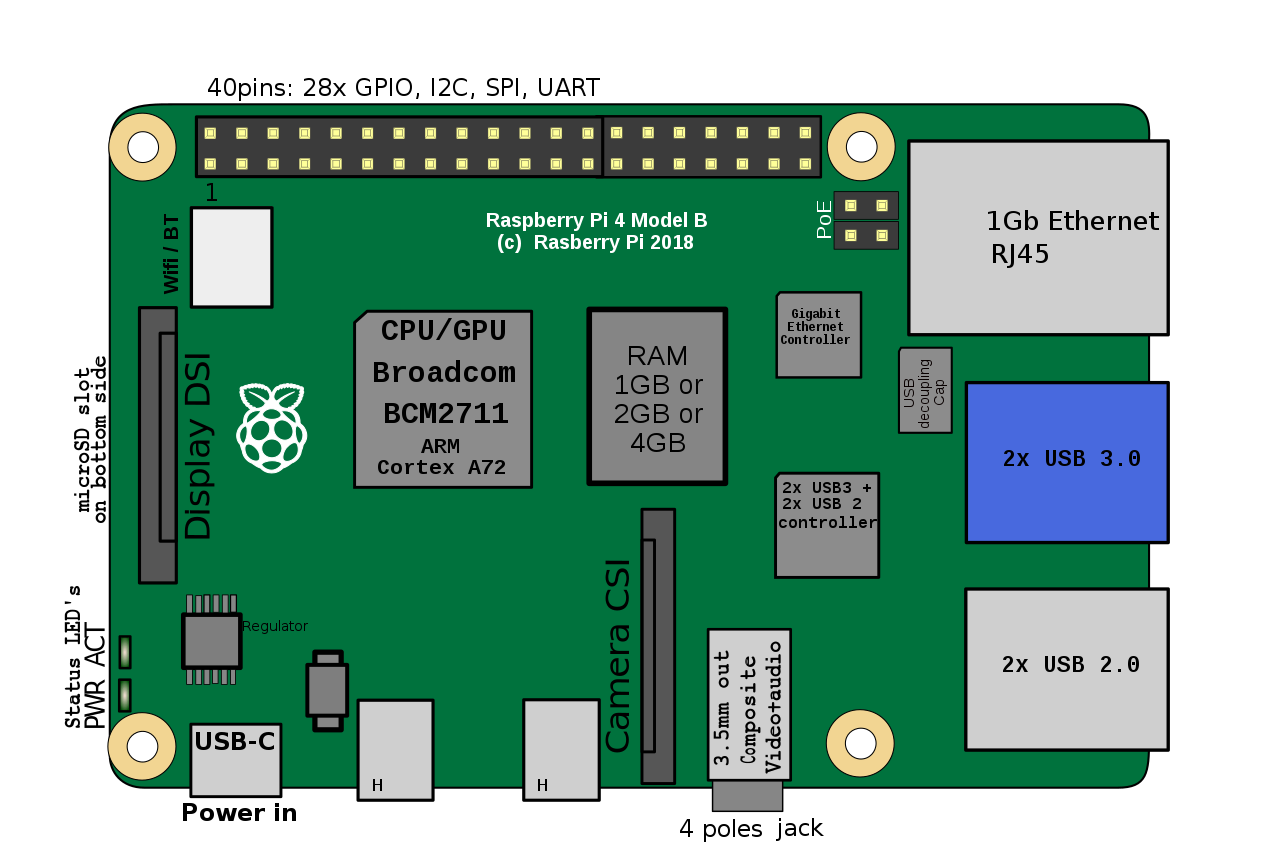
\includegraphics[width=10cm]{img/RaspberryPi_Model_4B.png}
\caption[Layout of Connectors and Main ICs on Raspberry Pi 4]{Layout of Connectors and Main ICs on Raspberry Pi 4\cite{rpidiag}}
\label{rpi}
\end{figure}

\subsubsection{Device Selection}

The selected device to implement the platform management system is the Raspberry Pi 4. As seen in Figure \ref{rpi}, the Raspberry Pi 4 is a small single-board computer that hosts a quad-core ARM Cortex A72 CPU, a CSI camera interface, 40 serial pins, Wi-Fi/Bluetooth, and a gigabit Ethernet port. We choose the Raspberry Pi 4 over other single-computer platforms (including Arduino/Beagleboard/Orange Pi) because the Raspberry Pi 4:

\begin{itemize}
\item is relatively inexpensive (CAN\$45 in November 2019),
\item has a large support community and a wealth of driver/library support,
\item supports a wide range of high throughput I/O standards (USB/WiFi/Ethernet/Serial, \textbf{C.EX.3}),
\item provides an industry-standard camera interface (\textbf{C.EX.5}),
\item supports extensible non-volatile storage (\textbf{F.CP.4}),
\item is presumed to have a cross-compatible successor (the Raspberry Pi 5) -- therefore future-proofing the PMB segment,
\item has an established community for technical support
\end{itemize} 

\subsubsection{Data Flow}
The overall data flow managed by the Raspberry Pi is as follows:
\begin{enumerate}
\item Video is acquired through the camera CSI interface
\item Frame manipulation/correction is performed on the video, if required by the specific machine learning use-case
\item Manipulated video is decomposed and transmitted over Ethernet to the programmable logic board (which performs the machine learning)
\item Machine learning results are received via Ethernet
\item Video, ML results, and system status information are transmitted via WiFi to the base station
\item (Optional) Results and video are stored locally on non-volatile storage for post-flight analysis
\end{enumerate}

All operations are managed by the ARM Cortex A72 chip running a headless version of the Raspbian operating system. 

\subsubsection{Use of Multiple Computing Boards}
The presence of on-board Wi-Fi and camera interfaces is the primary driving factor towards adopting a dual-board (PMB and PLB) solution. While a uni-board solution is possible, the development effort and cost of the computing platform would be considerably higher. Most programmable logic boards (including our chosen board, the Zedboard) require external expansion devices to interface with peripherals such as WiFi/cameras. These expansion devices, which connect to the programmable logic board via a serial connection, have poorly documented drivers and are of considerable expense -- ranging from US\$25 for a basic WiFi module\cite{digiwifi} to US\$200 for a compatible camera interface card\cite{digipmod}. External expansion devices also require considerable glue logic on the programmable logic board, potentially risking non-compliance with constraint \textbf{C.EX.2}.

An additional consideration in selecting the two-board design regards platform extensibility --- the client may desire to increase the programmable logic capabilities of the computing platform in the future, requiring a board swap. If a single-board solution is implemented, the client would be required to migrate \textit{all} hardware/software to the larger board, requiring them to devote considerable effort to debug driver issues. Additionally, external expansion devices are not necessarily compatible with all PLBs -- adding constraints to the client's board selection or requiring the purchase of new interface cards. By offloading the interfacing work to a distinct \textit{platform management} board, the client can easily replace the PLB without considerable redevelopment (fulfilling constraint \textbf{C.EX.4}). 

To emphasize, the use of multiple computing boards is a design decision derived from the current budgetary constraint to use \textit{off-the-shelf} components in the development of this device. Upon the completion of new hardware-accelerated machine learning implementations, the client may wish to integrate the capabilities of both boards into a single (custom ASIC) platform (at considerable expense). 

\subsubsection{Interface with Programmable Logic Board}

To interface with the PLB, data packets are sent via a bi-directional TCP/IP-managed Ethernet connection. TCP/IP over Ethernet was selected in lieu of serial solutions (such as I2C) as:
\begin{itemize}
\item Ethernet is equally as ubiquitous on modern programmable logic boards,
\item Ethernet has higher maximum throughput on modern platforms (on the Zedboard, 1 Gbps on Ethernet vs. 400 Kbps on serial)
\item Ethernet has more robust error control coding schemes (such as implicit forward error correction\cite{mclaughlin_warland}) compared to serial, leading to more reliable data transfer
\end{itemize} 

The selection of Ethernet over serial precludes the use of the \textit{Zero W} variant of the Raspberry Pi, as the Zero W does not provide Ethernet support. 
